\chapter{Neutrino Oscillation}
\label{ch:intro}

The study of neutrinos and their oscillations has been the source
of countless surprises in the development of the
Standard Model of particle physics and beyond.
Neutrinos are currently the only particles exhibiting properties
not explained by the Standard Model
which can be studied---not just searched for---on Earth in a laboratory setting.
This chapter will introduce the history of neutrinos (\cref{sec:history});
describe the modern theoretical understanding of neutrino oscillation
(\cref{sec:osc_intro});
and present the experimental techniques used to study neutrino oscillation,
focusing on those used by the Daya Bay Reactor Neutrino experiment (\cref{sec:experiment_intro}).

\section{History of neutrinos}
\label{sec:history}

The first evidence of neutrinos emerged in the form of
the continuous spectrum of $\beta$ particles
emitted during nuclear decay.
The continuous spectrum was first reported by Chadwick in 1914 \cite{chadwick_beta}.
Additional measurements confirming Chadwick's result accumulated over the next decade.
At the time, $\beta$ decay was thought to be a 2-body decay
of a nucleus $N$ with charge $Z$ and atomic mass $A$:
\begin{equation}\label{eq:old_beta}
    N(A, Z) \to N(A, Z+1) + \beta^-
\end{equation}
Conservation of energy uniquely determines the energy
of the outgoing $\beta$ particles for a given decay,
thus producing a monoenergetic spectrum,
as had been observed for $\alpha$ and $\gamma$ decays.
In 1931, rather than sacrifice the principle of conservation of energy,
Pauli proposed the introduction of a light neutral particle
produced during $\beta$ decay that escaped detection
due to a low interaction cross section \cite{pauli_letter}.
The particle, eventually named the neutrino ($\nu$) by Fermi,
provided the additional degree of freedom needed
to maintain conservation of energy and allow for a continuous $\beta$ spectrum
via the 3-body decay
\begin{equation}\label{eq:beta_mid}
    N(A, Z) \to N(A, Z+1) + \beta^- + \nu.
\end{equation}
Subsequent experiments, detailed below,
would reveal the existence of an antineutrino $\bar{\nu}$,
followed by a distinction between neutrino flavors $\nu_e, \nu_\mu,$
and, much later, $\nu_\tau$.
Lepton flavor conservation requires that
the original neutrino proposed to solve
the problem of the continuous $\beta$ spectrum
is actually the electron antineutrino (\nuebar).
Additionally, the discoveries of the proton and neutron
led to the conclusion that $\beta$ decay was the result of
the decay of a single neutron rather than of the nucleus as a whole.
The modern understanding of $\beta$ decay is therefore
\begin{equation}\label{eq:beta_modern}
    n \to p + e^- + \nuebar.
\end{equation}
This process and its equivalents for $\mu$ and $\tau$
provide the vast majority of opportunities for
experimental investigation of the neutrino to this day.

\subsection{Discovery of the neutrino}
\label{subsec:discovery}

Reines and Cowan were the first to observe the neutrino experimentally in 1956
\cite{reines_cowan}.
They used a liquid scintillator detector to monitor a target of
water with dissolved $\text{CdCl}_2$
placed near the Savannah River Plant nuclear reactor.
The neutrinos were expected to undergo the inverse beta decay (IBD) reaction,
\begin{equation}\label{eq:ibd}
    \nuebar + p \to n + e^+,
\end{equation}
with the proton supplied by a hydrogen nucleus (\isotope[1]{H}) in the water.
The positron would annihilate in the water almost immediately,
producing two $\gamma$ rays which were detected in the liquid scintillator
as a prompt signal.
The neutron would scatter within the target for a few ($\sim5$) \si{\us}
and eventually capture on a Cd nucleus,
triggering the emission of several $\gamma$ rays totalling \SI{9}{\MeV},
detected as a delayed event by the liquid scintillator.
IBD events were identified by the coincidence of a prompt and delayed event
at a rate of \SI[per-mode=reciprocal]{2.88\pm0.22}{\per\hour},
only present when the reactor was powered on.
This experiment was the earliest progenitor of the Daya Bay experiment,
which also observes reactor \nuebar{} using a liquid scintillator detector
and the principle of the prompt-delayed coincidence for IBD events.

\subsection{Difference between \texorpdfstring{$\nu$ and $\bar{\nu}$}{nu and nu-bar}}
\label{subsec:nu_vs_nubar}

Even prior to Reines and Cowan's observation of the neutrino,
Davis was able to provide convincing evidence that
the antineutrino was different from the neutrino \cite{davis_diff_nuebar}.
In 1954, Davis attempted to observe the reaction
\begin{equation}\label{eq:davis_nubar}
    \isotope[37]{Cl} + \bar{\nu} \to \isotope[37]{Ar} + \beta^-.
\end{equation}
If $\nu=\bar{\nu}$, then lepton number conservation could be violated
and the reaction could occur.
A tank containing \SI{3900}{\liter} of $\text{CCl}_4$
was placed in close proximity to the Brookhaven nuclear reactor.
Any \isotope[37]{Ar} produced was extracted using helium gas,
and the resulting gas was monitored using a Geiger counter
to observe the decay of \isotope[37]{Ar} (half-life 35 days).
No decays of \isotope[37]{Ar} were observed over the expected background.
Thus it was concluded that $\nu\neq\bar{\nu}$.

Davis noted in the conclusion of his report that the same experimental setup
could be used to detect neutrinos produced by the sun.
This experiment will be discussed later as the earliest evidence
for neutrino oscillations.

\subsection{Helicity of the neutrino}
\label{subsec:helicity}

The helicity of the neutrino was measured by
Goldhaber, Grodzins and Sunyar in 1957 \cite{helicity_measurement,helicity_review}.
The kinematics of the reaction chain
\begin{align}\label{eq:lampshade}
    \begin{split}
        e^- + \isotope[152m]{Eu}(0^-) \to \nu_e
        + & \isotope[152]{Sm}^*(1^-) \\
          & \isotope[152]{Sm}^*(1^-) \to \isotope[152]{Sm}(0^+) + \gamma
    \end{split}
\end{align}
ensure that if the final $\gamma$-ray is emitted
in exactly the opposite direction as the emitted $\nu_e$,
then they will have the same helicity.
Since those $\gamma$-rays of interest
are also maximally Doppler boosted by the recoil of the $\isotope[152]{Sm}^*(1^-)$,
a system was devised to only accept the highest-energy $\gamma$-rays.
Specifically, only the $\gamma$-rays which had been Doppler boosted
would be able to excite the same nuclear state in a separate sample of
$\text{Sm}_2\text{O}_3$,
through a process known as resonant fluorescence or resonant scattering.
$\gamma$-rays emitted at any other angle would suffer from energy loss
due to recoil effects
and thus would not be able to excite the same energy level in a separate nucleus.
A NaI scintillation counter was placed behind shielding
so that only $\gamma$-rays which were scattered by the $\text{Sm}_2\text{O}_3$
would be detected (\cref{fig:lampshade}).

The helicity of the emitted $\gamma$ rays was measured
using an electromagnet surrounding the \isotope[152m]{Eu} source.
When the electrons in the magnet were polarized in a particular direction,
only $\gamma$ rays with the opposite polarization (spin)
would Compton scatter off them.
By comparing the number of resonant scatters $N_\uparrow$
using an upward-pointing magnetic field
with the number $N_\downarrow$ from a downward-pointing field,
the polarization, and therefore the helicity, could be measured.
With the field pointing up, the polarized electron spins point down,
and therefore a downward-traveling $\gamma$ ray
would only scatter if it had a upward-pointing spin, i.e. helicity $-1$.
Conversely, downward-traveling $\gamma$ rays
with helicity $-1$ are preferentially transmitted
when the field is pointing down.
Only the transmitted $\gamma$ rays have the opportunity to
resonantly scatter off the $\text{Sm}_2\text{O}_3$
and be detected by the NaI counter.
A measured excess of
\begin{equation}\label{eq:helicity_meas}
    \frac{N_{\downarrow}-N_{\uparrow}}{(N_{\downarrow}+N_{\uparrow})/2} =
    \num{0.017\pm0.003}
\end{equation}
was observed,
indicating that the $\gamma$ rays, and therefore the neutrino,
had helicity $-1$.

%allows for a connection between the helicity (polarization)
%of the emitted $\gamma$
%with the helicity of the $\nu_e$, which is not directly detected,
%as follows.
%The total inital momentum is approximately 0.
%Therefore the decay products $\nu_e$ and $\isotope[152]{Sm}^*(1^-)$
%must have equal and opposite momenta.
%Similarly, the initial angular momentum (including spin) is $\pm\nicefrac{1}{2}$,
%and the daughter nucleus is known to have spin 1,
%therefore the spins of the decay products must point in opposite directions.
%Since both decay products have spins and momenta in opposite directions,
%they must have the same helicity.
%When the $\isotope[152]{Sm}^*(1^-)$ decays,
%occasionally the $\gamma$ will be emitted in the same direction
%as the momentum of the parent nucleus (recoiling against the $\nu_e$).
%In this case, since the final state of the \isotope[152]{Sm} has spin 0,
%the $\gamma$ must have the same spin and direction of momentum
%as the parent $\isotope[152]{Sm}^*$ and therefore the same helicity as the $\nu_e$.
%If the $\gamma$ is emitted in a different direction,
%it has a nonzero probability of having the opposite helicity.
%A method was required to select only those $\gamma$ rays which
%were emitted in the same direction as the momentum of the parent nucleus
%to ensure they had the same helicity as the emitted $\nu_e$.

\begin{figure}
    \centering
    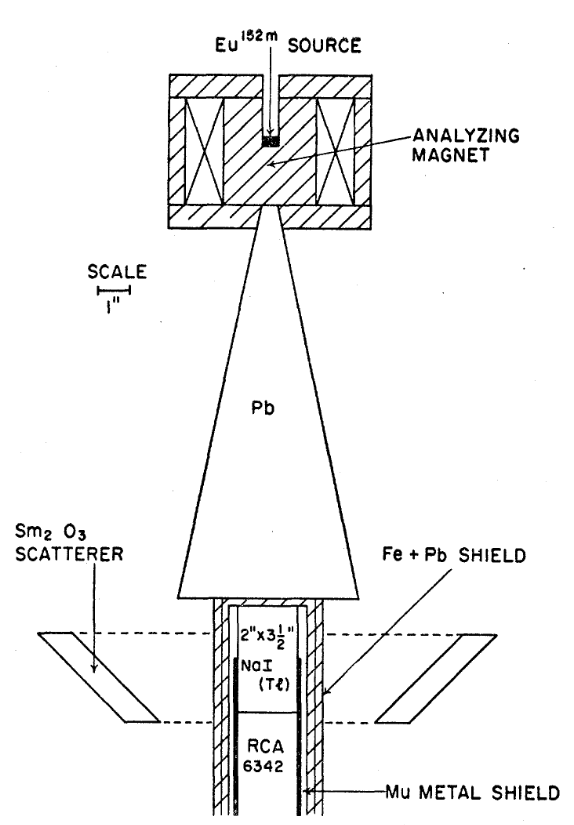
\includegraphics[width=0.38\textwidth]{ch_introduction/helicity_setup}
    \caption{
        Schematic layout of the experiment which measured
        the helicity of the neutrino \cite{helicity_measurement}.
    }
    \label{fig:lampshade}
\end{figure}

%A solution was found in the form of resonant fluorescence,
%the absorption and re-emission of a $\gamma$ ray
%by a nucleus with an energy level equal to that of the $\gamma$ ray.
%An obvious choice for this setup was the exact same isotope of $\isotope[152]{Sm}$,
%so target of $\text{Sm}_2\text{O}_3$
%containing \SI{26.8}{\percent} \isotope[152]{Sm}
%was placed in a ring below the sample of \isotope[152]{Eu}
%(\cref{fig:lampshade}).
%The $\gamma$ rays which resonantly scattered on the $\text{Sm}_2\text{O}_3$
%were detected using a NaI scintillation counter.
%This arrangement selected only the desired $\gamma$ rays
%(those emitted in the same direction as the parent nucleus)
%due to the following properties of resonant fluorescence:
%The emitted $\gamma$ rays are in general
%slightly (\SI{\sim3}{\eV}) below the energy
%needed to re-excite the same mode in a target nucleus
%due to the recoil during absorption.
%The $\gamma$ rays emitted in exactly the same direction
%as the parent $\isotope[152]{Sm}^*$
%experince a recoil on emission which takes the form of
%a Doppler shift to higher energy
%(due to the parent's own recoil against the $\nu_e$).
%Even the additional energy from the maximal Doppler shift
%was not sufficient to cause the resonant fluorescence;
%only when coupled with the random thermal motion
%of both the parent and target nuclei
%was there a non-negligible probability of interaction.
%Thus the $\gamma$ rays reaching the NaI counter
%must have been resonantly scattered off the target \isotope[152]{Sm};
%therefore they must have been emitted in exactly the same direction
%as the parent $\isotope[152]{Sm}^*(1-)$,
%carrying the same helicity as the $\nu_e$
%that caused the initial recoil.



\subsection{Discovery of neutrino flavors}
\label{subsec:nu_flavors}

In 1962, Schwartz, Lederman, \emph{et~al.} used the
Alternating Gradient Synchrotron (AGS) at Brookhaven
to demonstrate that $\nu_\mu$ behaved differently from $\nu_e$
\cite{numu_vs_nue}.
In the world's first accelerator neutrino experiment,
they produced a beam of $\nu_\mu$ by directing
the \SI{15}{\GeV} AGS proton beam
onto a fixed beryllium target and relying on the following reaction chain:
\begin{align}\label{eq:accel_reaction_chain}
    \begin{split}
        p + \text{Be} \to &\pi^{\pm} + X \\
        &\pi^{\pm} \to \mu^{\pm} + \nu(\bar{\nu}) \\
    \end{split}
\end{align}
A series of spark chambers of total target mass \SI{10}{\tonne}
was exposed to the neutrino beam,
with the non-neutrino beam products attenuated
by \SI{13.5}{\m} of steel shielding.
In a universe with only one type of neutrino (and one type of antineutrino),
the neutrino beam would have produced equal quantities
of electrons and muons.
After an exposure of \num{3.48e17}~protons ($\sim300$~hours),
a total of 113 events were observed,
of which 56 were identified as muon-like single-track or vertex events
(5 of which were statistically attributed to contamination by cosmic rays),
8 were electron-like electromagnetic showers, and 49 were background.
The electron-like events were attributed to
kaon contamination in the beam,
and, in any event, were not consistent with the
expected energy distribution of events due to the
primary muon-associated neutrino beam.
With dozens of muon events and not a single electron event
attributable to the muon-associated neutrinos,
it was concluded that $\nu_\mu \neq \nu_e$.


\subsection{Discovery of the neutral current}
\label{subsec:neutral_current}

The unified electroweak theory proposed independently by
Glashow \cite{glashow}, Weinberg \cite{weinberg} and Salam \cite{salam}
in the 1960s
predicted the existence of a weak neutral current (NC)
carried by a massive boson named the Z,
which would not change neutrinos into charged leptons and vice versa.
Thus a signature of a neutral current interaction involving neutrinos
would be a single visible interaction product (e.g. an electron or nucleon),
with no visible incoming particle and no additional visible interactin products.

In 1973, the Gargamelle neutrino experiment at CERN
published observations of neutrino interactions
that did not produce a charged lepton,
thus proving the existence of the hadronic \cite{gargamelle,gargamelle_short}
and leptonic \cite{gargamelle_leptonic} neutral current (NC) weak interactions.
The Gargamelle bubble chamber contained \SI{\sim10}{\tonne} of
$\text{CF}_3\text{Br}$ within a \SI{2}{\tesla} magnetic field.
It was exposed to a neutrino beam which could switch
between $\nu_\mu$ and $\bar{\nu}_\mu$ modes.
The search for leptonic NC interactions selected was designed
to identify events of the form
\begin{equation}\label{eq:leptonic_neutral_current}
    \nu_\mu(\bar{\nu}_\mu) + e^- \to \nu_\mu(\bar{\nu}_\mu) + e^-.
\end{equation}
After scanning \num{375000} $\nu$-mode interaction images
and \num{360000} $\bar{\nu}$-mode images,
one NC event was found in a $\bar{\nu}$-mode image,
shown in \cref{fig:gargamelle}.

The search for hadronic NC interactions selected events of the form
\begin{align}\label{eq:neutral_current}
    \begin{split}
        \nu_\mu(\bar{\nu}_\mu) + \text{N} &\to \nu_\mu(\bar{\nu}_\mu)
        + \text{hadrons (NC), and} \\
        \nu_\mu(\bar{\nu}_\mu) + \text{N} &\to \mu^-(\mu^+) + \text{hadrons (CC)}.
    \end{split}
\end{align}
The CC interactions were used to calibrate the detection and particle ID (``scanning'')
efficiencies of the detector.
A total of 102 $\nu$- and 64 $\bar{\nu}$-induced interactions were observed
with the NC signature of only hadrons as interaction products,
and no associated $\mu$.
A typical NC event image is shown in \cref{fig:gargamelle}.
These neutrino interactions were the first experimental evidence
of the weak neutral current and Z boson,
and the first experimental validation of a prediction of
the unified electroweak theory.


\begin{figure}
    \centering
    \begin{subfigure}{0.49\textwidth}
        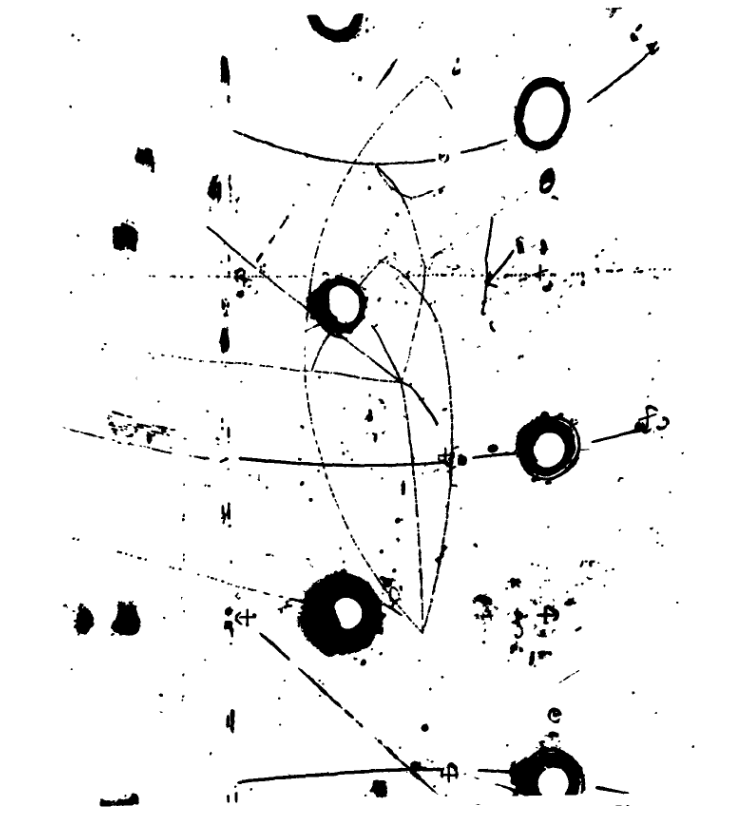
\includegraphics[width=\textwidth]{ch_introduction/gargamelle_hadronic}
    \end{subfigure}
    \begin{subfigure}{0.49\textwidth}
        \includegraphics[width=\textwidth]{ch_introduction/gargamelle_leptonic}
    \end{subfigure}
    \caption{
        Photographs of a hadronic NC interaction (left, \cite{gargamelle})
        and the first observed leptonic NC interaction
        (right, \cite{gargamelle_leptonic_image})
        taken by the Gargamelle neutrino experiment.
    }
    \label{fig:gargamelle}
\end{figure}

\subsection{The solar neutrino problem}
\label{subsec:homestake}

When Davis concluded the experiment which determined that $\nu\neq\bar{\nu}$,
he noted that the same experimental principle could be used
to search for neutrinos produced by the sun \cite{davis_diff_nuebar}.
This would provide experimental validation of the Standard Solar Model (SSM),
which describes the nuclear fusion processes
that are the source of the sun's energy.
The SSM predictions for neutrino fluxes (\cref{fig:solarflux})
were computed by Bahcall,
who worked closely with Davis \cite{bahcall2004}.
A tank of \SI{610}{\tonne} of $\text{CCl}_4$
located in the Homestake gold mine in South Dakota
was used as a target for the reaction
\begin{equation}\label{eq:davis_nu}
    \isotope[37]{Cl} + \nu_e \to \isotope[37]{Ar} + \beta^-.
\end{equation}
This reaction has a threshold of \SI{0.814}{\MeV} \cite{solar_review}
and is accessible primarily to neutrinos
produced via \isotope[8]{B} decay in the sun.
Helium gas was fed through the tank
to collect the \isotope[37]{Ar},
which was then extracted from the helium
and monitored with a proportional counter,
with each decay corresponding to a single neutrino interaction \cite{homestake1968}.
The experiment began in 1965 and released results periodically
until it shut down in 1992.

\begin{figure}
    \centering
    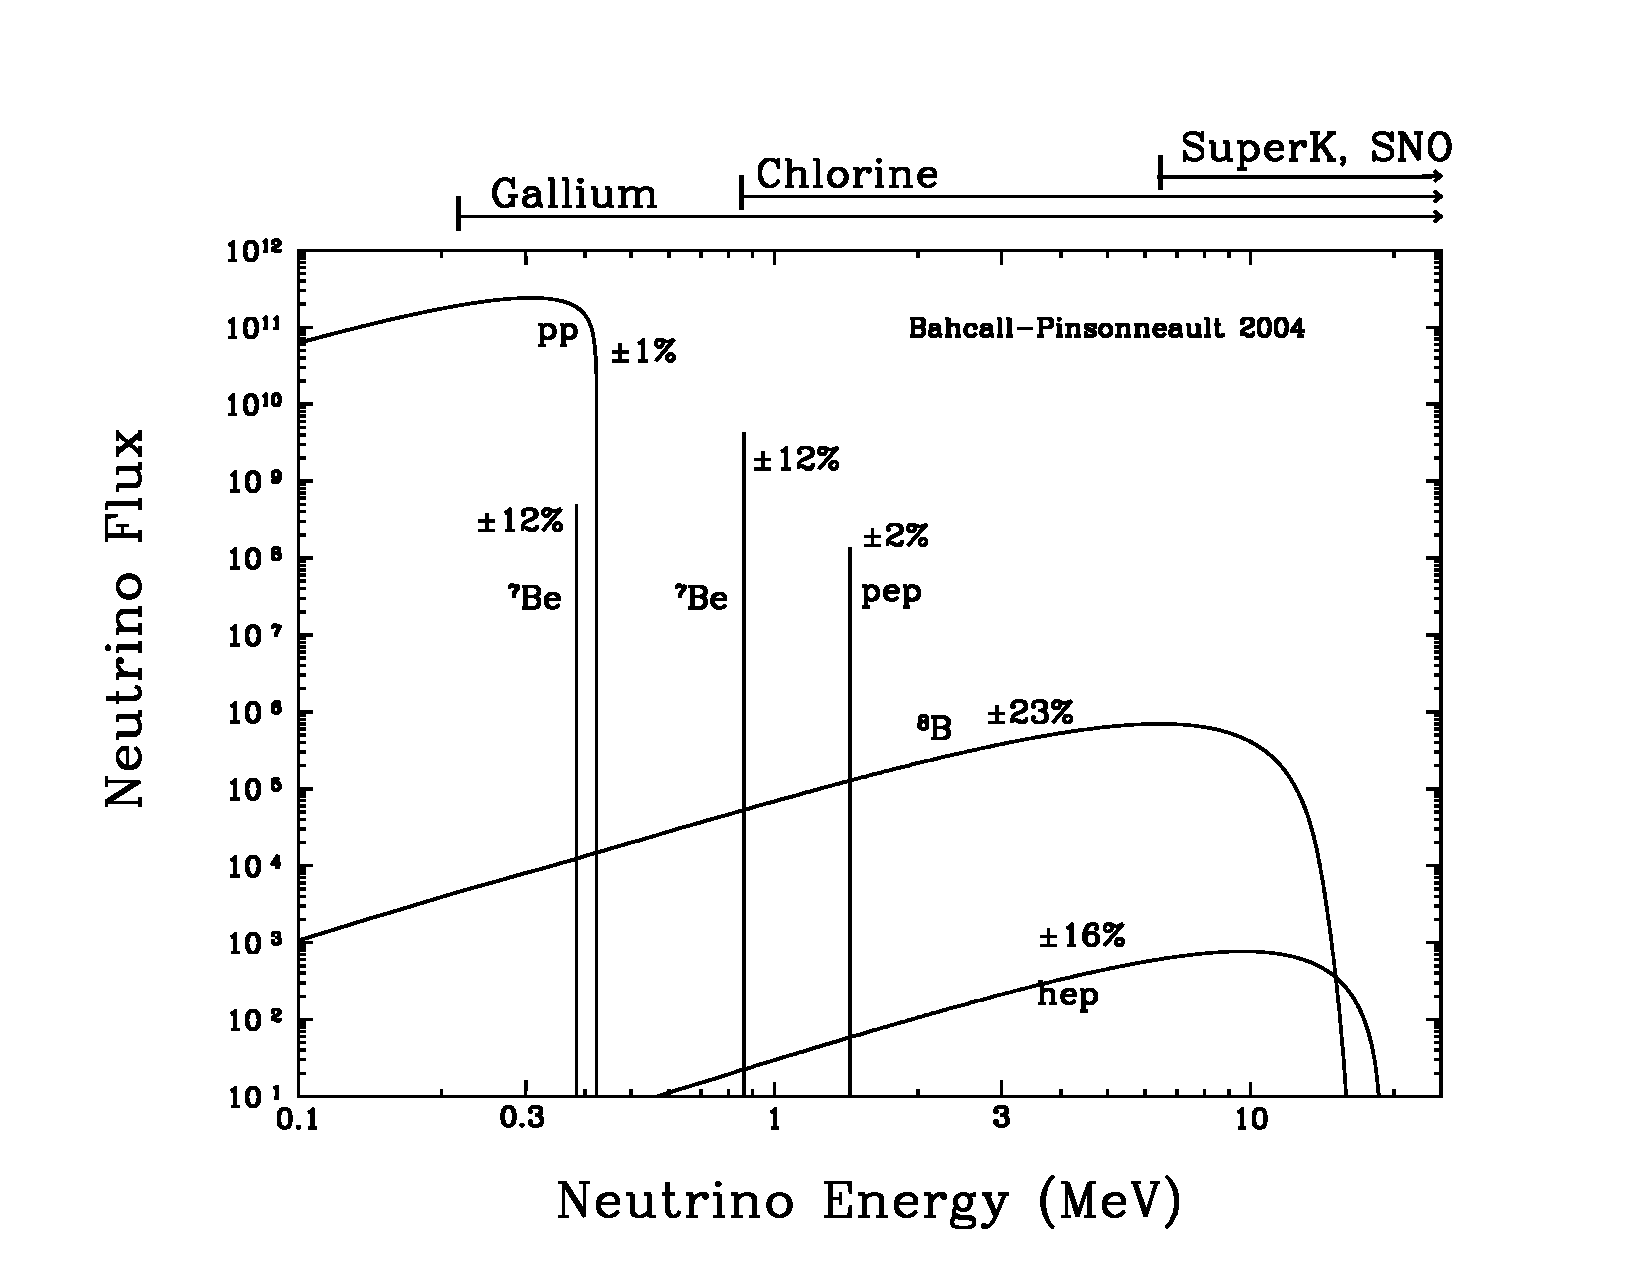
\includegraphics[width=0.8\textwidth]{ch_introduction/solar_spectrum}
    \caption{
        Predicted solar neutrino fluxes according to the SSM \cite{bahcall2004}.
        The units of neutrino flux are
        \si[per-mode=reciprocal]{\per\square\cm\per\second} for monoenergetic processes
        and \si[per-mode=reciprocal]{\per\square\cm\per\second\per\MeV}
        for continuous processes.
        The quoted percentages represent the uncertainty
        on the normalization of the flux for the corresponding process.
    }
    \label{fig:solarflux}
\end{figure}

Even in the early published results,
the experiment observed a substantial deficit of neutrino events
compared to the prediction from the SSM.
Results were expressed in solar neutrino units (SNU),
with $\SI{1}{\SNU} = 1$ interaction per second per $10^{36}$ target nuclei.
In 1968, no significant number of events above background was observed;
the limit of no more than \SI{3}{\SNU} was compared to a prediction of
\SI{20\pm12}{\SNU} \cite{homestake1968}.
After more than a decade of observation,
the prediction and observation had evolved to \SI{5.8\pm2.2}{\SNU}
and \SI{2.1\pm0.3}{\SNU}, respectively,
and the discrepancy had become known as the ``solar neutrino problem.''
The two remaining routes for resolving the discrepancy were
(1) errors in the SSM, and (2) that neutrinos ``oscillate or decay''
between their production in the sun and their detection on Earth \cite{davis1985}.

\begin{figure}
    \centering
    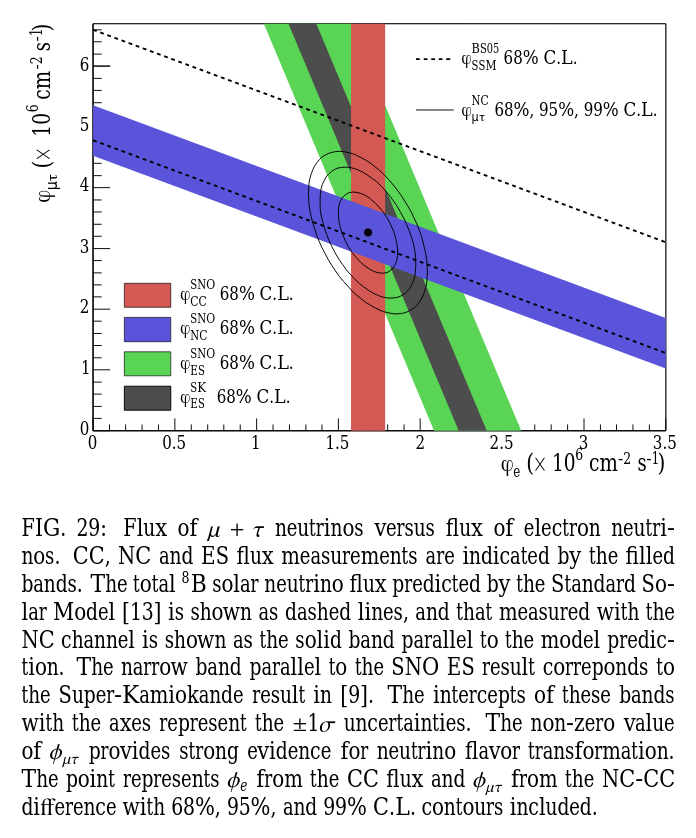
\includegraphics[width=0.8\textwidth]{ch_introduction/sno_salt}
    \caption{
        Measured fluxes of solar $\nu_e$ and ``solar'' $\nu_{\mu,\tau}$
        constrained by SNO (Phases I and II) and Super-Kamiokande,
        compared to the SSM prediction \cite{sno_salt2004}.
    }
    \label{fig:sno_plots}
\end{figure}

\begin{figure}
    \centering
    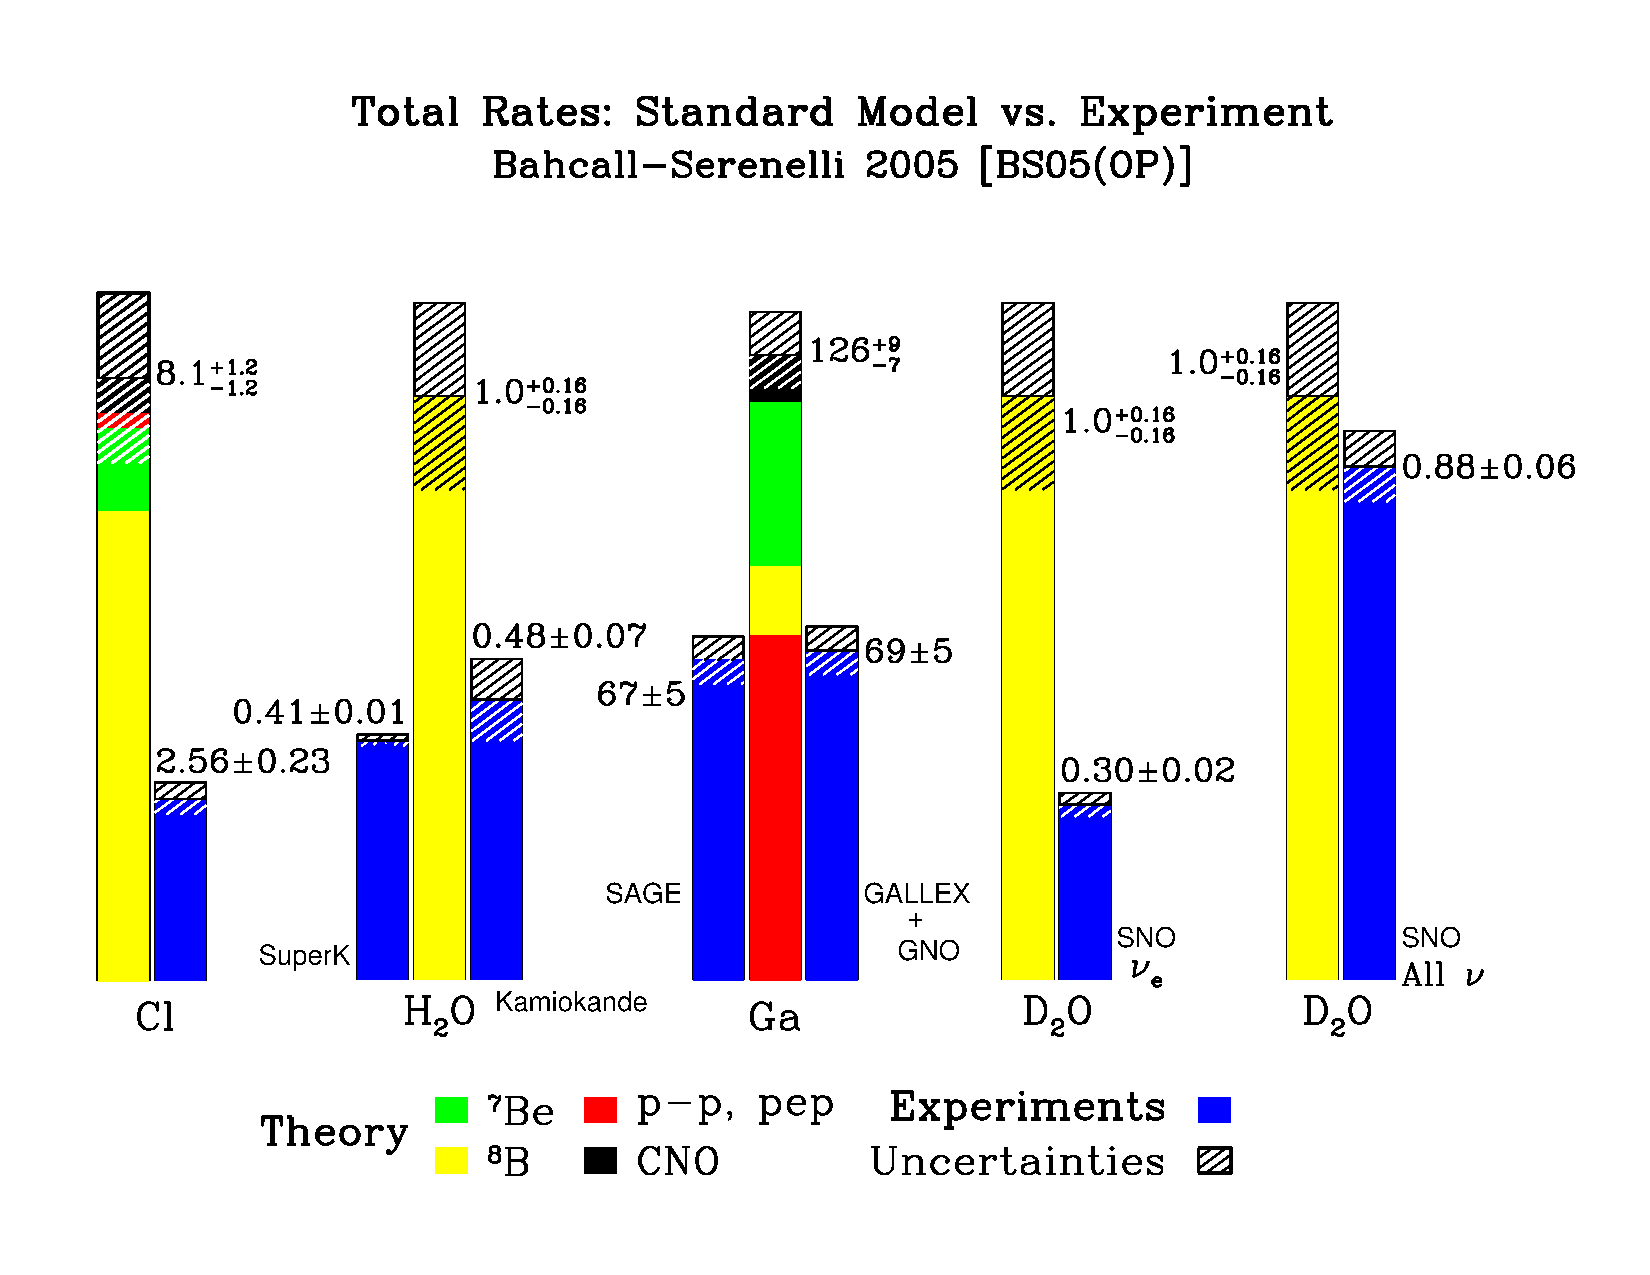
\includegraphics[width=0.7\textwidth]{ch_introduction/solar_resolution}
    \caption{
        Predictions and measurements for \isotope[37]{Cl}, \isotope[71]{Ga},
        $\text{H}_2\text{O}$, and $\text{D}_2\text{O}$ solar neutrino experiments.
        Taken from \cite{bahcall_images} based on \cite{bahcall2005_diagram}.
    }
    \label{fig:solar_neutrino_fixed}
\end{figure}

Davis and others supported the construction of
new experiments based on the same radiochemical principle,
but using the reaction
\begin{equation}\label{eq:gallium}
    \isotope[71]{Ga} + \nu_e \to \isotope[71]{Ge} + \beta^-,
\end{equation}
which has a substantially lower threshold
of \SI{0.233}{\MeV} (cf. \SI{0.814}{\MeV} for \isotope[37]{Cl})
and thus is sensitive not just to \isotope[8]{B} neutrinos
but also those from \isotope[7]{Be} and the $pp$ and $pep$ fusion cycles in the sun.
The SAGE and GALLEX/GNO experiments observed deficits of approximately \SI{50}{\percent}
compared to the SSM prediction \cite{sage,gallex}.
The discrepancy between the \SI{\sim33}{\percent} deficit
in the \isotope[37]{Cl} experiment
and the \SI{50}{\percent} deficit in the \isotope[71]{Ga} experiments
added additional layers to the solar neutrino problem.
Separately, the Kamiokande-II and Kamiokande-III experiments,
which used an $\text{H}_2\text{O}$ target
and photomultiplier tubes (PMTs)
to detect Cherenkov radiation from the energetic electron produced by
\begin{equation}\label{eq:kamiokande}
    \nu_e + p \to n + e^-,
\end{equation}
also observed \SI{\sim50}{\percent} of the SSM-predicted solar neutrino flux
\cite{kamiokande_III}.
The experiment's ability to assign a timestamp and direction to each neutrino event
also led to the first direct confirmation that these neutrinos
actually originated from the sun:
the outgoing $e^-$ tended to point away from the sun,
no matter the time of day or year.

The Sudbury Neutrino Observatory (SNO) definitively resolved
the solar neutrino problem in 2001 in favor of neutrino oscillations,
validating the SSM as an accurate model of the processes powering the sun
\cite{sno2001}.
The experiment monitored \SI{1}{\tonne} of heavy water ($\text{D}_2\text{O}$)
surrounded by a spherical array of photomultiplier tubes (PMTs)
which detect the Cherenkov radiation produced by neutrino interaction products.
The use of heavy water, first proposed by Chen in 1984 \cite{chen_d2o},
allowed SNO to observe both charged-current (CC)
and neutral-current (NC) interactions,
and thus compare the flux of solar $\nu_e$ with the total $\nu$ flux
from the sun over all flavors.
The three interaction categories for SNO were
\begin{align}\label{eq:sno_interactions}
    \begin{split}
        \nu_e + \isotope[2]{H} & \to e^- + p + p \text{ (CC)} \\
        \nu_x + \isotope[2]{H} & \to \nu_x + n + p  \text{ (NC)}\\
                               & \text{with }n + \isotope[2]{H} \to
                               \isotope[3]{H} + \gamma (\SI{6.26}{\MeV})
                               \text{ (Phase I),} \\
                               & n + \isotope[35]{Cl} \to
                               \isotope[36]{Cl} + \text{ multiple }\gamma\text{'s}
                               (\SI{8.6}{\MeV})
                               \text{ (Phase II), or} \\
                               & n + \isotope[3]{He} \to
                               \isotope[3]{H} + p \text{ (Phase III)}\\
        \nu_x + e^- & \to \nu_x + e^- \text{ (elastic scatter (ES))}
    \end{split}
\end{align}
In these reactions $\nu_x$ means any flavor of neutrino ($x = e,\mu,\tau$).
Elastic scatter reactions could occur via CC (for $\nu_e$ only, and with a higher cross section)
or via NC (for all flavors including $\nu_e$).
The three phases of the experiment differed in the technique
used to detect the neutron produced by the NC interaction.
In Phase I, the target medium was pure $\text{D}_2\text{O}$.
In Phase II, salt (NaCl) was dissolved in the target
since \isotope[35]{Cl} has a much higher neutron capture cross section
than \isotope[2]{H}, and also produces higher-energy $\gamma$-rays \cite{sno_salt2004}.
In Phase III, the NaCl was removed
and proportional counters containing \isotope[3]{He}
were deployed to provide a complementary measurement of the NC channel
with mostly-independent systematic uncertainties \cite{sno_ncd_instrumentation}.
SNO reproduced the existing deficits using the CC interaction category,
corroborating the observation of missing solar $\nu_e$.
The NC observation included all neutrino flavors and matched the SSM prediction,
as did the ES measurement.
All of the neutrinos predicted by the SSM did reach Earth,
but only some of them interacted as $\nu_e$: thus their flavors had changed.
Comparisons of $\nu_e$ with $\nu_{\mu,\tau}$ fluxes
from SNO (Phases I and II) and Super-Kamiokande are shown in \cref{fig:sno_plots}.
A summary diagram of the solar neutrino problem and its resolution by SNO
is shown in \cref{fig:solar_neutrino_fixed}.

The KamLAND experiment performed
an independent measurement of electron (anti)\-neutrino disappearance
by observing reactor antineutrinos (\SI{\sim3}{\MeV}) from all over Japan
at an average baseline of \SI{\sim180}{\km},
with the first results announced in 2002 \cite{kamland_first}.
Observations indicated significant distortion
in the energy spectrum of \nuebar{} events,
as shown in \cref{fig:kamland_spec}.
The specific shape of the distortion
matched the predictions of the three-flavor oscillation model
described in \cref{subsec:theory}.

\begin{figure}
    \centering
    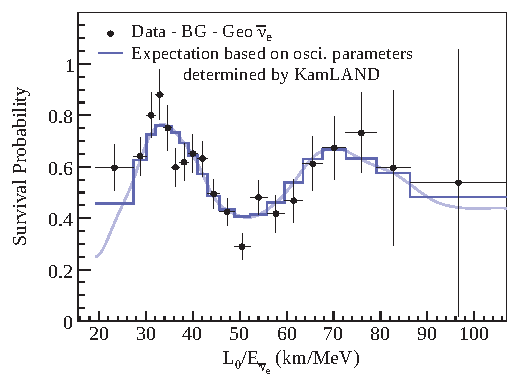
\includegraphics[width=0.8\textwidth]{ch_introduction/kamland2008}
    \caption{
        Spectrum of \nuebar{} events at KamLAND.
        The substantial trough around $L_0/E_{\bar{\nu}_e} = \SI{50}{\km\per\MeV}$
        was a signature of neutrino oscillation.
    }
    \label{fig:kamland_spec}
\end{figure}

\subsection{The atmospheric neutrino anomaly}
\label{subsec:atmospheric_anomaly}

Though the earliest signs of neutrino disappearance and oscillations
were discovered in the solar neutrino sector,
a parallel history exists in observations of atmospheric neutrinos.
Atmospheric neutrinos are secondary decay products of
collisions of cosmic rays (mostly protons) with nuclei in the atmosphere.
Among the most common primary decay products are $\pi^{\pm}$,
which undergo the decay $\pi^+ \to \mu^+ + \nu_\mu$ and its CP conjugate.
The daughter muons then decay via $\mu^+ \to \bar{\nu_\mu} + e^+ + \nu_e$
and its CP conjugate.
Thus for energies low enough that all muons decay before they reach the ground,
the expected ratio of $\nu_\mu$ to $\nu_e$ fluxes should be about 2.
The precise expectation can be computed with a Monte Carlo simulation
that incorporates knowledge of the atmosphere and of the kinematics of
pion, kaon and muon decays \cite{neutrino_textbook}.

In 1988, the Kamiokande experiment observed muon and electron-type
atmospheric neutrino events and compared their rates to a Monte Carlo prediction.
The rate of electron-type neutrino events matched the prediction,
but the rate of muon-type events was only \SI{59\pm7}{\percent}
of the rate predicted by the Monte Carlo simulation,
as shown in \cref{fig:kamioka_atmo} \cite{kamiokande_atmo}.
The IMB experiment observed fluxes broadly consistent with
the reports from Kamiokande \cite{imb_atmo}.

\begin{figure}
    \centering
    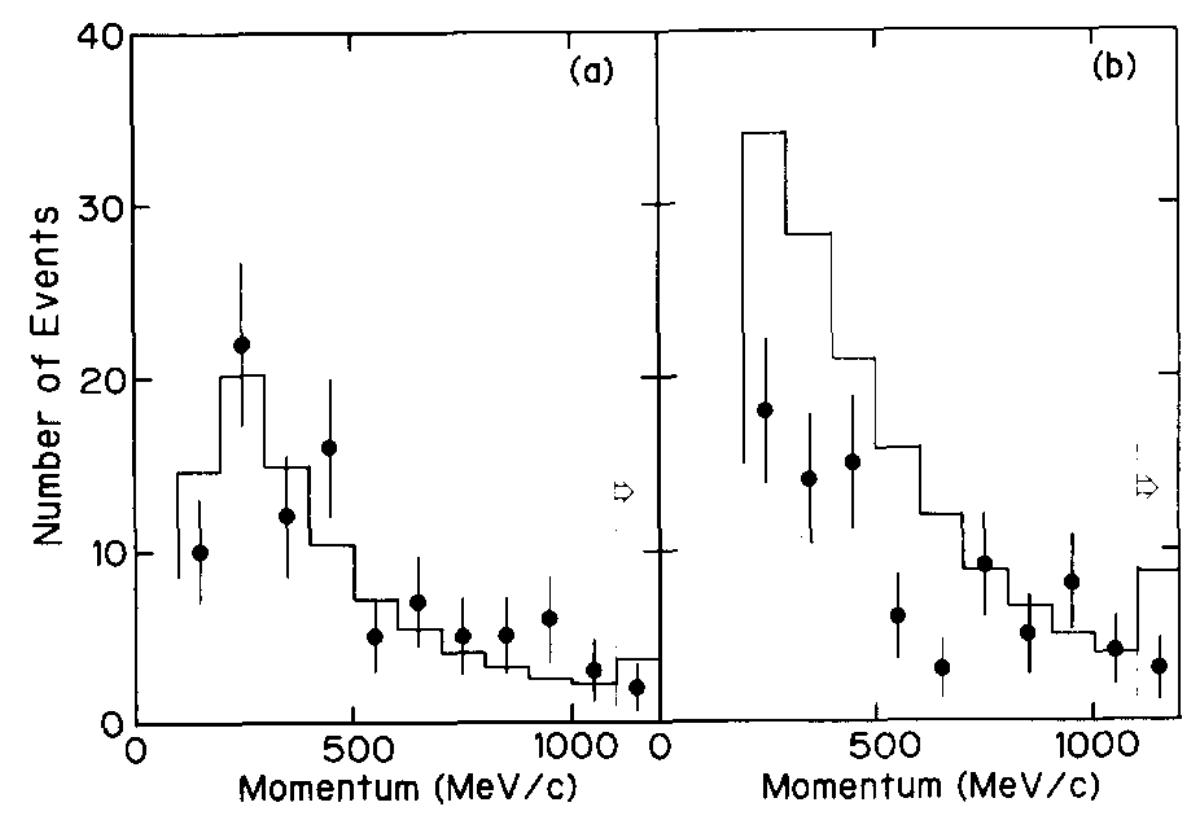
\includegraphics[width=0.6\textwidth]{ch_introduction/kamioka_atmo_spec}
    \caption{
        Momentum spectra for electron-like (left) and muon-like (right) events
        at the Kamiokande detector \cite{kamiokande_atmo}.
        The electron-like distribution is consistent with the Monte Carlo prediction,
        but the muon-like distribution has substantially fewer events
        than predicted.
    }
    \label{fig:kamioka_atmo}
\end{figure}

Super-Kamiokande, the \SI{50}{\kilo\tonne} successor experiment to Kamiokande,
provided the resolution
to the atmospheric anomaly in 1998
by comparing the flux of upward-going neutrinos
to that of downward-going neutrinos.
The fluxes were predicted to be independent of zenith angle
by a convenient property of spherical geometry
assuming only that the cosmic ray flux was uniform around the Earth,
which is true for cosmic rays with energy above a few \si{\GeV}
(energetic enough to be unaffected by the geomagnetic field).
Thus neutrino fluxes over different baselines
could be compared directly to each other
in a model-independent manner, rather than
just to Monte Carlo predictions.
The experiment observed a deficit of upward-going atmospheric $\nu_\mu$
relative to the rate of downward-going $\nu_\mu$ \cite{superk1998}.
The upward-going neutrinos were produced on the opposite side of the Earth
and so traveled farther than the downward-going neutrinos.
Since negligibly few neutrinos scattered as they propagated through the Earth,
this result proved that atmospheric $\nu_\mu$ oscillate to other flavors
as they travel.
The measured distribution of zenith angles for electron and muon neutrino events
at Super-Kamiokande is shown in \cref{fig:superk_zenith}.
Super-Kamiokande also performed measurements of the solar neutrino flux
which matched the results from Kamiokande.
\cite{superk_solar1998,superk_solar2001}.

\begin{figure}
    \centering
    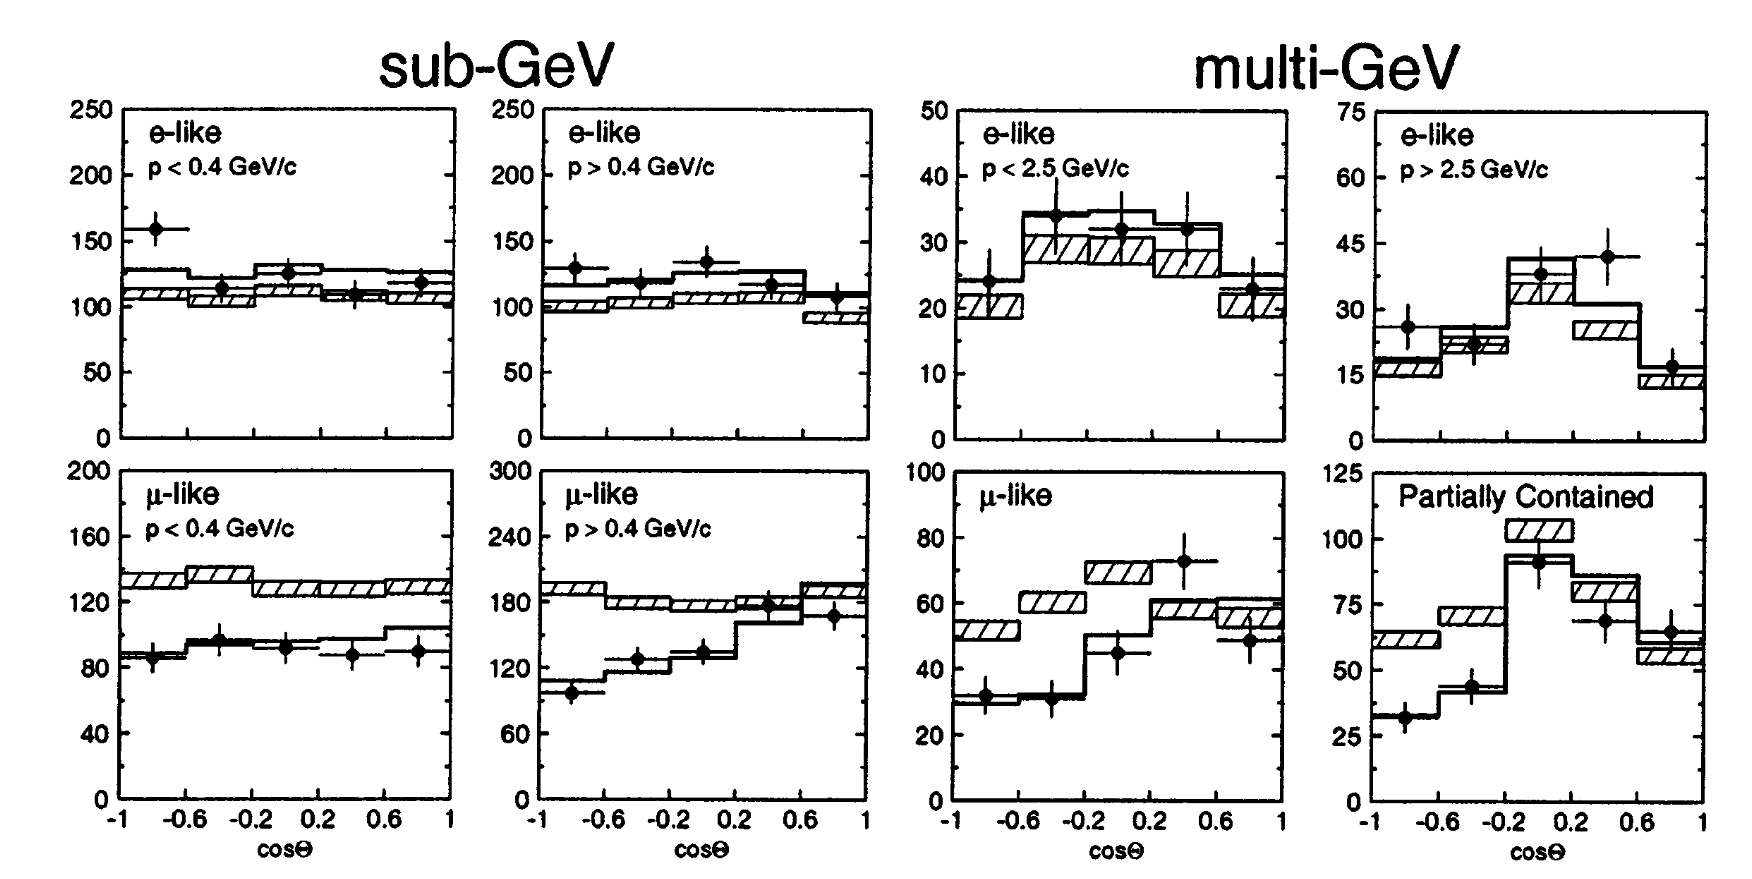
\includegraphics[width=\textwidth]{ch_introduction/superk_zenith_dist}
    \caption{
        Distributions of zenith angle at the Super-Kamiokande experiment
        \cite{superk1998}.
        These distributions show that $\nu_\mu$'s which were produced farther away
        ($\cos\Theta < 0$)
        were more likely to disappear, presumably by oscillating to $\nu_\tau$.
    }
    \label{fig:superk_zenith}
\end{figure}


\section{Neutrino oscillation}
\label{sec:osc_intro}

The Standard Model of particle physics (SM)
describes neutrinos as the massless electroweak partners
to the left-handed charged leptons $e_L,\mu_L,\tau_L$.
The observation of neutrino oscillation provided proof that,
like for quarks, neutrino flavor eigenstates are not
eigenstates of the Hamiltonian (``energy eigenstates''),
and further, that neutrinos have nonzero mass.
In \cref{subsec:theory}, the theoretical formalism for neutrino oscillation is discussed.
The specific solutions for two- and three-neutrino mixing
are presented in \cref{subsec:two_nu_mixing,subsec:three_nu_mixing},
respectively.
\Cref{subsec:osc_param_exp} describes the experiments which measured
each oscillation parameter
except for \thetaot{}, which is the focus of \cref{sec:experiment_intro}.
When describing the phenomenology of Majorana neutrinos
as well as the matter effect that governs solar neutrino behavior,
the more general phrase ``neutrino mixing''
is often used instead of ``neutrino oscillation''
since in both of these systems
the neutrino states are not described by oscillatory probability amplitudes.

\subsection{Oscillation theory}
\label{subsec:theory}

In the following, $c = \hbar = 1$ unless otherwise noted.
This derivation follows those presented in \cite{neutrino_textbook}
and \cite{huang_thesis}.
In a generic theory with $n$ leptonic flavors,
each charged lepton $l_\alpha^-$ is paired with
an associated neutrino $\nu_\alpha$.
The association is realized via the charged current (CC) interaction vertex
connecting $W, l_\alpha,$ and $\nu_\alpha$.
The neutrino state participating in this interaction
is known as the $\alpha$ flavor eigenstate, notated $\ket{\nu_\alpha}$.
In general, the flavor eigenstates will not be equal to the energy eigenstates
$\ket{\nu_i}$
(which are eigenstates of the Hamiltonian and have definite mass).
The relation between the mass and flavor eigenstates can be written as
\begin{align}\label{eq:general_eigenstates}
    \begin{split}
        \ket{\nu_\alpha} &= \sum_{i=1}^n U^*_{\alpha i} \ket{\nu_i} \\
        \ket{\nu_i} &= \sum_{\alpha\in\set{\text{flavors}}} U_{\alpha i} \ket{\nu_\alpha}
    \end{split}
\end{align}
where $U$ is a unitary matrix known as the mixing matrix.
The components of this equation obey the following unitarity relations:
\begin{align}\label{eq:unitarity}
    \begin{split}
        \braket{\nu_\alpha | \nu_\beta} &= \delta_{\alpha\beta} \\
        \braket{\nu_i | \nu_j} &= \delta_{ij} \\
        U^\dagger U &= \mathbf{1}
    \end{split}
\end{align}

The mass eigenstates are eigenstates of the Hamiltonian,
$\hat{H}\ket{\nu_i(t)} = E_i\ket{\nu_i(t)}$,
thus Schroedinger's equation takes a simple form:
\begin{align}\label{eq:schroedinger}
    \begin{split}
        \hat{H}\ket{\nu_i(t)} = E_i\ket{\nu_i(t)} &= i\frac{d}{dt}\ket{\nu_i(t)} \\
        \implies \ket{\nu_i(t)} &= e^{-iE_it}\ket{\nu_i(0)}
    \end{split}
\end{align}
Defining $\ket{\nu_\alpha} = \ket{\nu_\alpha(0)}$,
the evolution of a flavor eigenstate can be expressed
using \cref{eq:general_eigenstates}:
\begin{align}\label{eq:state_evolution}
    \begin{split}
        \ket{\nu_\alpha(t)}
        &= \sum_{i=1}^n U^*_{\alpha i} e^{-iE_it}\ket{\nu_i} \\
        &= \sum_{i=1}^nU^*_{\alpha i} e^{-iE_it}
        \left(\sum_{\rho\in\set{\text{flavors}}} U_{\rho i} \ket{\nu_\rho}\right) \\
        &= \sum_i\sum_\rho U^*_{\alpha i} U_{\rho i} e^{-iE_it}\ket{\nu_\rho}
    \end{split}
\end{align}
The amplitude $A_{\alpha\to\beta}(t)$
for observing the state $\ket{\nu_\beta}$ after
a neutrino produced as $\ket{\nu_\alpha}$ evolves over time $t$
is computed as the overlap
\begin{align}\label{eq:osc_amplitude}
    \begin{split}
        A_{\alpha\to\beta}(t) = \braket{\nu_\beta | \nu_\alpha(t)}
        &= \bra{\nu_\beta} \sum_i\sum_\rho U^*_{\alpha i} U_{\rho i}
        e^{-iE_it}\ket{\nu_\rho} \\
        &= \sum_i U^*_{\alpha i} U_{\beta i} e^{-iE_it} \\
    \end{split}
\end{align}
The probability for observing $\ket{\nu_\alpha(t)}$ in state $\ket{\nu_\beta}$
is simply the amplitude squared:
\begin{align}\label{eq:oscprob_general}
    \begin{split}
        P_{\alpha\to\beta}(t) = \left|A_{\alpha\to\beta}(t)\right|^2
        &= \left|\sum_i U^*_{\alpha i} U_{\beta i} e^{-iE_it}\right|^2 \\
        &= \left(\sum_iU_{\alpha i} U^*_{\beta i} e^{iE_it}\right)
        \left(\sum_j U^*_{\alpha j} U_{\beta j} e^{-iE_jt}\right) \\
        &= \sum_i\sum_j U^*_{\alpha j} U^*_{\beta i} U_{\alpha i} U_{\beta j}
        e^{-i(E_j - E_i)t}
    \end{split}
\end{align}
All (currently) experimentally-accessible neutrinos are ultrarelativistic,
i.e. $p \gg m$.
Thus the energy can be approximated as
\begin{align}\label{eq:energy_approx}
    \begin{split}
        E_i = \sqrt{p^2 + m_i^2}
        &= p\sqrt{1 + \frac{m_i^2}{p^2}} \\
        &\approx p\left(1 + \frac{m_i^2}{2p^2}\right) = p + \frac{m_i^2}{2p} \\
        &\approx E + \frac{m_i^2}{2E},
    \end{split}
\end{align}
where $E$ is the energy that a massless neutrino would have with momentum $p$.
An assumption is made that the three ``components'' $\ket{\nu_i}$
of the neutrino state $\ket{\nu_\alpha}$
were produced with the same momentum $p$ but slightly different energies $E_i$.
This assumption is in general poorly justified,
but for the fact that the resulting equations are validated by experiments.
In any event, this approximation yields the identity
\begin{equation}\label{eq:msq_approx}
    E_j - E_i \approx \frac{m_j^2 - m_i^2}{2E}.
\end{equation}
The established framework for computing oscillation probabilities
using these approximations, known as the plane-wave formalism,
is applicable over an extraordinarily wide
kinematic parameter space despite the unusual assumption.
A more general wave-packet formalism avoids these concerns
at the expense of additional mathematical machinery,
and reaches the same conclusions for all current experiments.
For a detailed discussion of the wave-packet formalism see
\cite[Ch.~8 of][]{neutrino_textbook}.

Continuing on by applying \cref{eq:msq_approx} to \cref{eq:oscprob_general}
with the ultrarelativistic approximation $t \approx L$
and the definition $\Delta m^2_{ij} = m_i^2 - m_j^2$,
\begin{align}\label{eq:oscprob_general_2}
    \begin{split}
        P_{\alpha\to\beta}(L)
        &= \sum_{ij} U^*_{\alpha j} U^*_{\beta i} U_{\alpha i} U_{\beta j}
        e^{i\frac{\Delta m^2_{ij}}{2E}L}
    \end{split}
\end{align}
This expression can be simplified by grouping the terms where $i=j$
and those where $i\neq j$.
When $i=j$, $\Delta m^2_{ij} = 0$.
For $i\neq j$, the matrix elements and the phase term can each be written
as the sum of real and imaginary parts and multiplied together term-by-term.
The final (real) probability contains contributions from both
the real and imaginary parts but as desired is purely real:
\begin{align}\label{eq:oscprob_general_3}
    \begin{split}
        P_{\alpha\to\beta}(L) =
        & \sum_i \left|U_{\alpha i}\right|^2 \left|U_{\beta i}\right|^2 \\
        & + 2\sum_{i>j} \Re \left[
            U^*_{\alpha j} U^*_{\beta i} U_{\alpha i} U_{\beta j}
        \right]
        \cos\left(\Delta m^2_{ij}\frac{L}{2E}\right) \\
        & + 2\sum_{i>j} \Im \left[
            U^*_{\alpha j} U^*_{\beta i} U_{\alpha i} U_{\beta j}
        \right]
        \sin\left(\Delta m^2_{ij}\frac{L}{2E}\right) \\
    \end{split}
\end{align}
with $\Re$ and $\Im$ denoting the real and imaginary parts (respectively)
of a complex number.
To simplify further, the leading term can be rewritten
using the unitarity relation:
\begin{align}\label{eq:sub_unitarity}
    \begin{split}
        \delta_{\alpha\beta}
        &= (U^\dagger U)^2_{\alpha\beta} \\
        &= \sum_{ij} U^*_{\alpha j} U^*_{\beta i} U_{\alpha i} U_{\beta j} \\
        &= \sum_i \left|U_{\alpha i}\right|^2 \left|U_{\beta i}\right|^2
        + 2\sum_{i>j} \Re \left[
            U^*_{\alpha j} U^*_{\beta i} U_{\alpha i} U_{\beta j}
        \right]
    \end{split}
\end{align}
Substituting \cref{eq:sub_unitarity} into \cref{eq:oscprob_general_3},
the general formula for oscillation probability for $n$ neutrinos is obtained:
\begin{align}\label{eq:oscprob_general_final}
    \begin{split}
        P_{\alpha\to\beta}(L) =
        &\ \delta_{\alpha\beta} \\
        & - 4\sum_{i>j} \Re \left[
            U^*_{\alpha j} U^*_{\beta i} U_{\alpha i} U_{\beta j}
        \right]
        \sin^2\left(\Delta m^2_{ij}\frac{L}{4E}\right) \\
        & + 2\sum_{i>j} \Im \left[
            U^*_{\alpha j} U^*_{\beta i} U_{\alpha i} U_{\beta j}
        \right]
        \sin\left(\Delta m^2_{ij}\frac{L}{2E}\right) \\
    \end{split}
\end{align}
In the special case where $\alpha = \beta$, the probability
is known as the survival probability.
The product of matrix elements
$U^*_{\alpha j} U^*_{\beta i} U_{\alpha i} U_{\beta j}$
becomes manifestly real,
hence the imaginary term in \cref{eq:oscprob_general_final} is zero,
yielding the general formula for survival probability:
\begin{equation}\label{eq:survival_prob_general}
        P_{\text{sur}} = P_{\alpha\to\alpha}(L) =
        1 - 4\sum_{i>j}
        \left|U_{\alpha i}\right|^2
        \left|U_{\alpha j}\right|^2
        \sin^2\left(\Delta m^2_{ij}\frac{L}{4E}\right) \\
\end{equation}
The phase of the oscillation, often abbreviated as $\Delta_{ij}$,
can be rewritten in physical units by
inserting the dimensionful values for $c$ and $\hbar$:
\begin{equation}\label{eq:osc_phase_shorthand}
    \Delta_{ij} = \Delta m^2_{ij}\frac{L}{4E} \to
    \Delta m^2_{ij} c^4 \frac{L}{4\hbar cE}
    \approx 1.267
    \frac{\Delta m^2_{ij}}{(\SI{1}{\eV}/c^2)^2}
    \frac{L}{\SI{1}{\m}}
    \frac{\SI{1}{\MeV}}{E}
\end{equation}

When considering oscillations of antineutrinos ($\bar{\nu}$)
from (anti-)flavor $\bar{\alpha}$ to $\bar{\beta}$,
the only difference is that the complex conjugate
of the unitary mixing matrix is used,
leading to an identical result for survival probability,
and a slightly-altered result for the general case,
\begin{align}\label{eq:oscprob_general_anti}
    \begin{split}
        P_{\bar{\alpha}\to\bar{\beta}}(L) =
        &\ \delta_{\alpha\beta} \\
        & - 4\sum_{i>j} \Re \left[
            U^*_{\alpha j} U^*_{\beta i} U_{\alpha i} U_{\beta j}
        \right]
        \sin^2\left(\Delta m^2_{ij}\frac{L}{4E}\right) \\
        & - 2\sum_{i>j} \Im \left[
            U^*_{\alpha j} U^*_{\beta i} U_{\alpha i} U_{\beta j}
        \right]
        \sin\left(\Delta m^2_{ij}\frac{L}{2E}\right), \\
    \end{split}
\end{align}
where the application of the complex conjugate does not affect
the real part of the product of matrix elements,
and changes only the sign of the imaginary part.

\subsection{Two-neutrino mixing}
\label{subsec:two_nu_mixing}

Before addressing the three-flavor oscillation phenomenology,
it is helpful to consider the two-flavor case,
which is both easier to understand
and also a good approximation to the oscillation behavior
of atmospheric $\nu_\mu$.
The $2\times2$ mixing matrix is purely real
and has only a single physical degree of freedom.
It has the form
\begin{equation}\label{eq:2d_mixing}
    U_{2\times2} =
    \begin{pmatrix}
        \cos\theta & \sin\theta \\
        -\sin\theta & \cos\theta
    \end{pmatrix},
\end{equation}
where $\theta$ is known as the mixing angle.
Since this matrix is purely real,
there is no difference between the neutrino and anti-neutrino
oscillation equations, preserving CP symmetry.
The two flavors are denoted $\alpha$ and $\beta$,
and the two mass states 1 and 2 with mass difference $\Delta m^2$.
The probability of a neutrino produced in the $\ket{\nu_\alpha}$ state
being observed as $\nu_\beta$ is then
\begin{equation}\label{eq:2d_osc}
    P_{\alpha\to\beta} = 4\cos^2\theta\sin^2\theta
    \sin^2\left(\Delta m^2_{ij}\frac{L}{4E}\right)
    = \sin^22\theta \sin^2\left(\Delta m^2_{ij}\frac{L}{4E}\right),
\end{equation}
and the survival probability is
\begin{equation}\label{eq:2d_p_sur}
    P_{\alpha\to\alpha} = 1 -
    \sin^22\theta \sin^2\left(\Delta m^2_{ij}\frac{L}{4E}\right),
\end{equation}
satisfying $P_{\alpha\to\beta} + P_{\alpha\to\alpha} = 1$ as expected.
These equations provide an intuitive meaning to the paramter $\theta$:
if $\theta = 0$, no oscillation will occur;
if $\theta = \nicefrac{\pi}{4}$,
then at the oscillation maximum, the neutrino will have a \SI{100}{\percent}
probability for being observed as a $\nu_\beta$.
This latter case is known as maximal mixing.
In the three-flavor scenario that describes the current understanding
of neutrino oscillation,
atmospheric neutrinos are observed to undergo near-maximal mixing
of the form $\nu_\mu\leftrightarrow\nu_\tau$,
with very little probability to transition to $\nu_e$,
corresponding to the relevant mixing angle being close to $\nicefrac{\pi}{4}$.

\subsection{Three-neutrino mixing}
\label{subsec:three_nu_mixing}

Three-neutrino mixing has a much more diverse phenomenology
than the simpler two-neutrino case
due to the additional degrees of freedom for a $3\times3$ unitary matrix.
The neutrino mixing matrix is known as the PMNS matrix,
named for Pontecorvo, Maki, Nakagawa and Sakata.
There are many different parametrizations of such a matrix,
but the one most convenient in describing neutrino oscillation is
\begin{equation}\label{eq:pmns}
    U_{\text{PMNS}} =
    \begin{pmatrix}
        1 & 0 & 0 \\
        0 & c_{23} & s_{23} \\
        0 & -s_{23} & c_{23}
    \end{pmatrix}
    \begin{pmatrix}
        c_{13} & 0 & s_{13}e^{-i\delta} \\
        0 & 1 & 0 \\
        -s_{13}e^{i\delta} & 0 & c_{13}
    \end{pmatrix}
    \begin{pmatrix}
        c_{12} & s_{12} & 0 \\
        -s_{12} & c_{12} & 0 \\
        0 & 0 & 1
    \end{pmatrix}
\end{equation}
where $s_{ij} = \sin\theta_{ij}$ for the three real mixing angles
$\theta_{12},\theta_{23}$, and $\theta_{13}$.
The complex phase $\delta$ is also known as $\delta_{CP}$
since CP violation is only possible if the PMNS matrix is complex,
i.e. $\delta_{CP} \notin \{0, \pi\}$.
The parametrization in \cref{eq:pmns} emphasizes the different oscillation regimes:
The first term is dominant for atmospheric neutrino oscillation,
with energies in the few \si{\GeV} range
and baselines of tens to thousands of \si{\km}.
The second term is dominant in reactor experiments
with energies in the few \si{\MeV} range
and baselines of \SI{\sim1}{\km},
and also in recent accelerator experiments
with both baselines and energies $\sim1000$ times higher.
The third term is dominant for solar neutrinos
and for reactor neutrinos at baselines of \SI{\sim100}{\km}.

The neutrino may be a Majorana particle.
If so, an additional two parameters %$\alpha_1$ and $\alpha_2$, the Majorana phases,
would govern the mixing between states.
They would appear as an additional factor in \cref{eq:pmns}
of the form $\text{diag}(e^{i\alpha_1}, e^{i\alpha_2}, 1)$.
These additional parameters cancel
during the derivation in \cref{subsec:theory}
and thus do not influence neutrino oscillation probabilities.

Mass state 1 is defined as the lighter of the two states
participating in solar neutrino oscillations,
and mass state 2 is the other relevant state.
Mass state 3 is the state which does not participate in solar neutrino oscillations.
The question of whether mass state 3 is heavier or lighter than the other two
is still unresolved;
this question is known as the neutrino mass ordering (or hierarchy) problem.
The normal ordering (NO) is $m_1 < m_2 < m_3 \Leftrightarrow \Delta m^2_{31} > 0$,
and the inverted ordering (IO) is
$m_3 < m_1 < m_2 \Leftrightarrow \Delta m^2_{31} < 0$.
For both mass orderings,
the mass splittings of the three neutrinos obey the sum rule
\begin{equation}\label{eq:sum_rule}
    \Delta m^2_{31} = \Delta m^2_{21} + \Delta m^2_{32}.
\end{equation}
The current measured values for all mixing parameters are \cite{pdg}
\begin{align}\label{eq:current_values}
    \begin{split}
        \sin^2\theta_{12} &= \num{0.307\pm0.013} \\
        \sin^2\theta_{23} &=
        \begin{cases}
            \num{0.545\pm0.021} & (\text{NO}) \\
            \num{0.547\pm0.021} & (\text{IO})
        \end{cases} \\
        \sin^2\theta_{13} &=
        \begin{cases}
            \num{2.18\pm0.07e-2} & (\text{global average}) \\
            (1.74^{+0.22}_{-0.24})\times10^{-2} & (\text{this work})
        \end{cases} \\
        \Delta m^2_{21} &= \SI{7.53\pm0.18e-5}{\eV\squared} \\
        \Delta m^2_{32} &=
        \begin{cases}
            \SI{2.453\pm0.034e-3}{\eV\squared} & (\text{NO}) \\
            -2.546^{+0.034}_{-0.040}\times 10^{-3}\,\si{\eV\squared} & (\text{IO})
        \end{cases} \\
        \delta_{CP} &= (\num{1.36\pm0.17})\times \SI{\pi}{\radian}\ (\text{NO})
    \end{split}
\end{align}
In this listing, the convention of reporting $\sin^2\theta_{ij}$
rather than $\sin^22\theta_{ij}$ was used
so that the octant of $\theta_{23}$
(whether it is greater than or less than \SI{45}{\degree})
is readily apparent.
At current experimental resolutions,
$\Delta m^2_{32}$ is still just barely indistinguishable from $\Delta m^2_{31}$,
given the above-quoted uncertainty in $\Delta m^2_{32}$ of
\SI{3.4e-5}{\eV\squared} compared to
a best-fit value for $\Delta m^2_{21}$ of \SI{7.53e-5}{\eV\squared}.

\begin{figure}
    \centering
    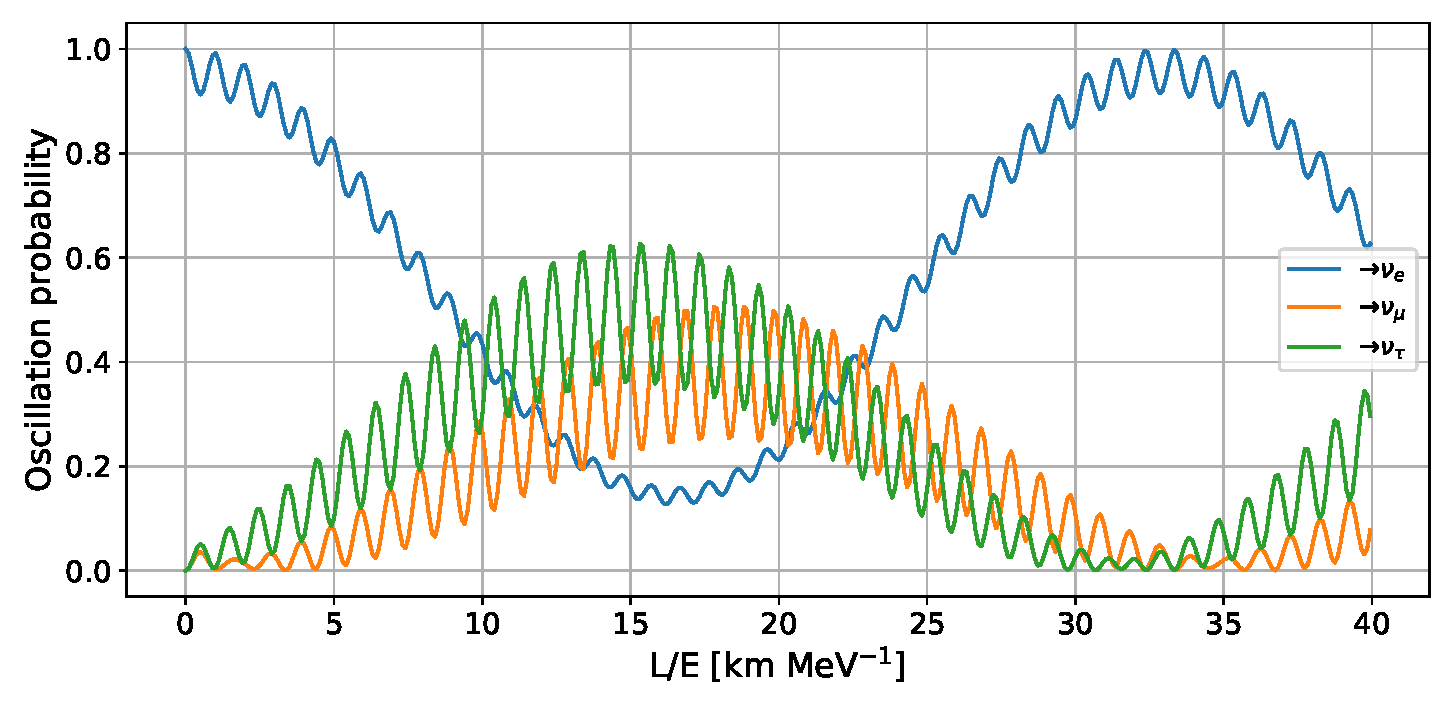
\includegraphics[width=\textwidth]{ch_introduction/oscprob_plot}
    \caption{
        Transition and survival probabilities for a neutrino
        with initial state $\ket{\nu_e}$
        using the current global average parameters
        assuming normal ordering (\cref{eq:current_values}).
        The high-frequency oscillations are governed by
        $\Delta m^2_{31}$ and $\Delta m^2_{32}$;
        the amplitude of the electron disappearance
        is controlled by \thetaot{} (the ``reactor angle''),
        and the ratio of $\nu_\mu$ to $\nu_\tau$
        is controlled by $\theta_{23}$ (the ``atmospheric angle'').
        The low-frequency oscillations are governed by
        $\Delta m^2_{21}$ and $\theta_{12}$ (the ``solar angle'').
    }
    \label{fig:oscprob}
\end{figure}

\subsection{Measurement of oscillation parameters}
\label{subsec:osc_param_exp}

\subsubsection{Solar parameters}
The solar parameters $\theta_{12}$ and $\Delta m^2_{21}$
were first measured using data from the aforementioned
Homestake/\isotope[37]{Cl}, SAGE, GALLEX/GNO, and SNO experiments.
The high matter densities in the sun impact the neutrino flavor transitions
through the Mikheyev-Smirnov-Wolfenstein (MSW) matter effect;
the so-called ``vacuum oscillation'' model described above
was not the dominant mechanism governing solar neutrinos,
though the two mechanisms share the same fundamental PMNS (mixing) matrix.
A detailed description of the measurements of $\theta_{12}$ and $\Delta m^2_21$ and the MSW effect
will be left to \cite{neutrino_textbook}.
Modern values for the solar parameters rely
on measurements from the Super-Kamiokande experiment.

The KamLAND experiment results (\cref{fig:kamland_spec})
were interpreted in the vacuum oscillation model
as measurements of the solar mixing parameters.
The agreement of the reactor antineutrino measurement from KamLAND
with the existing solar neutrino results
was a major success of the theory of neutrino mixing.
\Cref{fig:kamland_plus_solar} shows the constraints
from KamLAND using the vacuum oscillation framework
and from solar experiments using the MSW framework.

\begin{figure}
    \centering
    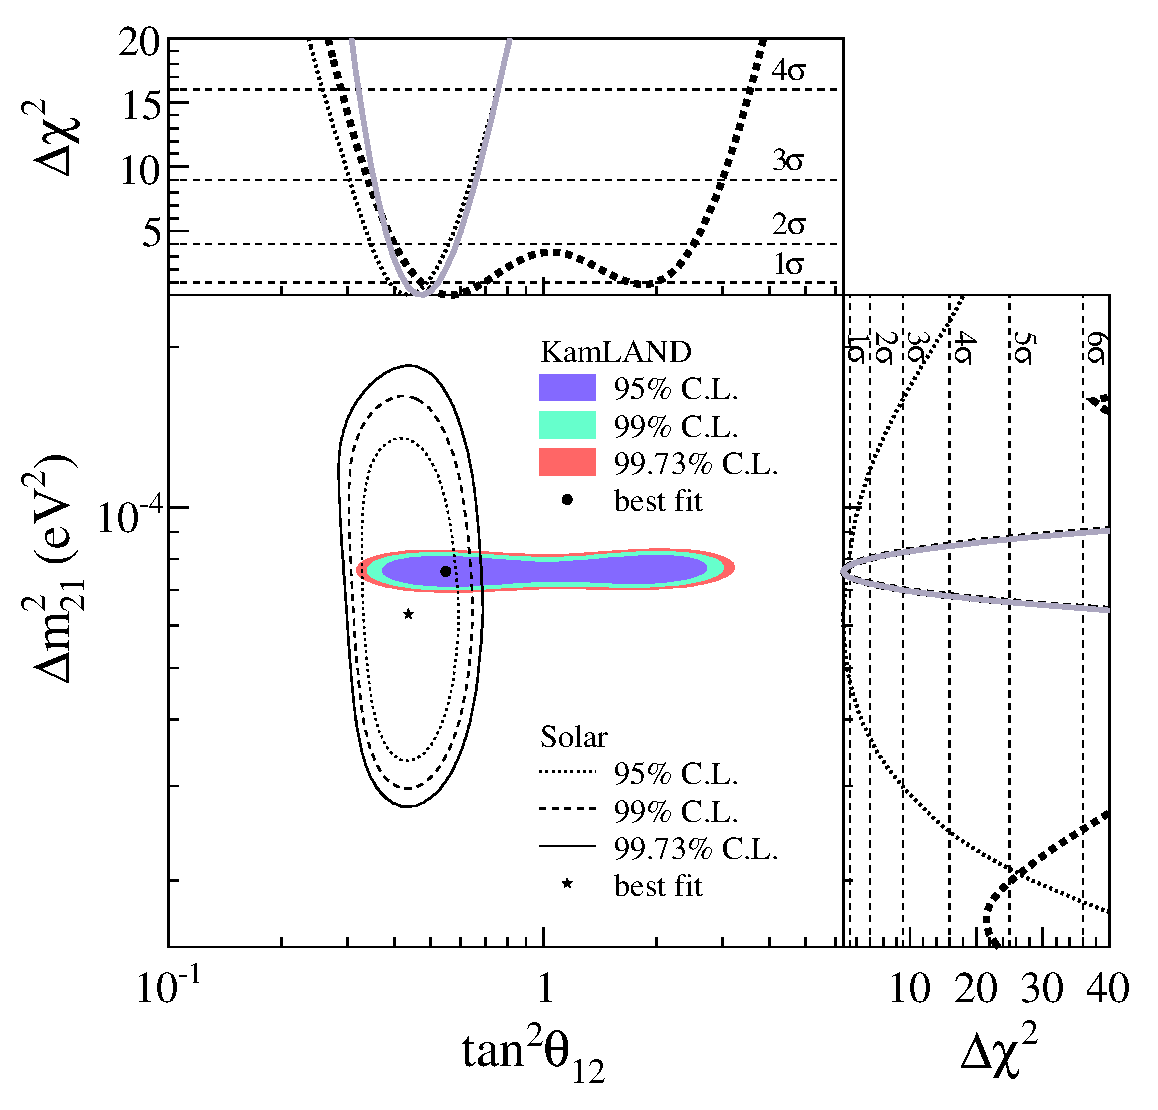
\includegraphics[width=0.7\textwidth]{ch_introduction/kamland_solar_fit}
    \caption{
        Allowed region for neutrino oscillation parameters from KamLAND and solar
        neutrino experiments.
        The side-panels show the $\Delta \chi^2$-profiles
        for KamLAND (dashed) and solar experiments (dotted) individually,
        as well as the combination of the two (solid).
        Figure and caption taken from \cite{kamland_latest}.
    }
    \label{fig:kamland_plus_solar}
\end{figure}

\subsubsection{Atmospheric parameters}
The Super-Kamiokande experiment measured $\theta_{23}$ and $\Delta m^2_{32}$
by comparing the rate of atmospheric neutrinos
traveling upward to those traveling downward
as described in \cref{subsec:atmospheric_anomaly}.
A nonzero up-down asymmetry of $-0.296\pm0.048(\text{stat.})\pm0.01(\text{syst.})$
was observed for muon-type events (including neutrinos and antineutrinos),
but the up-down asymmetry for electron-type events
of $-0.036\pm0.076\pm0.02$ was consistent with zero \cite{superk1998}.
Later investigations \cite{superk2004} showed the characteristic $\nicefrac{L}{E}$
dependence when comparing the observed muon-type events
to a Monte Carlo prediction,
with the distance traveled inferred from the zenith angle
(see \cref{fig:superk_l_over_e}).
The events used in the analysis had a reconstructed $\nicefrac{L}{E}$
with a resolution of \SI{<70}{\percent},
thus the characteristic shape of the $\nicefrac{L}{E}$ curve
was mostly washed out.
However, the location of the oscillation maximum
can be seen in \cref{fig:superk_l_over_e}
(where it appears as a minimum of surviving $\nu_\mu$),
providing the first measurement of $\Delta m^2_{32} = \SI{2.4e-3}{\eV\squared}$
Equally importantly, the asymptotic behavior
at large $\nicefrac{L}{E}$ reveals
the average value for the oscillation probability.
Since the average value is $\sim\nicefrac{1}{2}$,
the observation favored a value of $\sin^22\theta_{12} = 1$,
corresponding to maximal mixing.

\begin{figure}
    \centering
    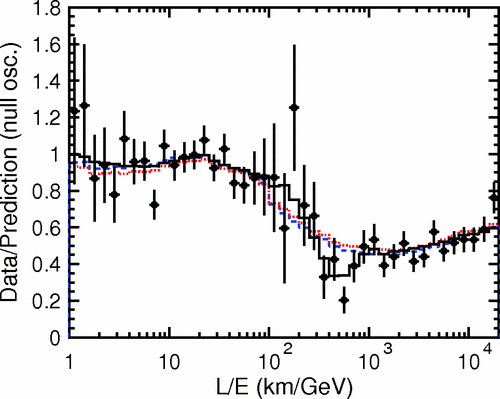
\includegraphics[width=0.6\textwidth]{ch_introduction/superk_atmo_l_over_e}
    \caption{
        Ratio of the data to the MC events without neutrino oscillation (points)
        as a function of the reconstructed L/E together with
        the best-fit expectation for 2-flavor $\nu_\mu\leftrightarrow\nu_\tau$
        oscillations (solid line).
        The error bars are statistical only.
        Also shown are the best-fit expectation for neutrino decay (dashed line)
        and neutrino decoherence (dotted line).
        Figure and caption taken from \cite{superk2004}.
    }
    \label{fig:superk_l_over_e}
\end{figure}

\subsubsection{Reactor parameter}
The measurement of the third mixing angle \thetaot{}
will be described in detail in \cref{sec:experiment_intro}.
This angle
governs the probability of $\nu_e$ (dis)appearance
at the atmospheric scale of $L/E \sim \SI{1}{\km\per\MeV}$
and is accessible by observing reactor \nuebar{} disappearance
and accelerator $\nu_e$ and \nuebar{} appearance.

\subsubsection{CP phase and mass ordering}
The final mixing parameter, $\delta_{CP}$,
is the subject of considerable current experimental effort.
Attempts to measure $\delta_{CP}$ involve
accelerator experiments comparing the rates of
$\nu_\mu\to\nu_e$ and $\bar{\nu}_\mu\to\bar{\nu}_e$ oscillations.
The current generation of experiments consists of
T2K, which utilizes the Super-Kamiokande detector,
and NOvA,
which uses a large segmented liquid scintillator detector \cite{nova_deltacp}.
The T2K experiment recently published evidence of $\delta_{CP}\neq 0$
at a significance of $3\sigma$ \cite{t2k_deltacp}.
These experiments provided the above-referenced measurement to $\delta_{CP}$
(\cref{eq:current_values}).
The next generation of experiments is currently under construction
and includes DUNE in the United States \cite{dune_potential}
and Hyper-Kamiokande in Japan \cite{hyperk2015}.

Two classes of experiments are sensitive to the neutrino mass ordering.
The first is the same accelerator experiments searching for $\delta_{CP}$;
the neutrino beams in these experiments travel substantial distances
through the Earth's crust,
which induces different distortions to the $\nu_e$ appearance spectrum
depending on the mass ordering.
The second class of experiments currently consists of
a single experiment under construction: JUNO \cite{junoproposal2016}.
Using similar technology to Daya Bay,
the JUNO experiment will perform a precise measurement
of the reactor \nuebar{} spectrum
at the $\Delta m^2_{21}$ oscillation maximum,
where the slight difference between
$\Delta m^2_{32}$ and $\Delta m^2_{31}$
will cause different effects depending
on which mass splitting is larger.
Current observations from accelerator experiments
agree better with normal ordering (NO)
predictions than with IO at the level of $2\sigma$ to $3\sigma$.

\section{Reactor neutrino experiments and \texorpdfstring{\thetaot}{theta13}}
\label{sec:experiment_intro}

As illustrated by \cref{fig:oscprob},
the probability of a transition of $\nu_e \leftrightarrow \nu_\mu$
or $\nu_e \leftrightarrow \nu_\tau$
has two characteristic wavelengths and amplitudes:
the larger is governed by $\theta_{12}$ and $\Delta m^2_{21}$,
while the smaller is governed by
$\theta_{13}$, $\Delta m^2_{32}$, and $\Delta m^2_{31}$
with a typical $\nicefrac{L}{E}$ scale of \SI{\sim0.5}{\km\per\MeV}.
The two experimentally-feasible signatures for \thetaot{}-governed oscillations
are $\nu_\mu\to\nu_e$ (appearance) and $\nu_e\to\nu_{\mu/\tau}$ (disappearance).
Appearance is most conveniently observed using accelerator neutrinos,
which are produced as a beam of primarily $\nu_\mu$ or $\bar{\nu}_\mu$.
Disappearance is easiest to observe using reactor \nuebar.

The survival probability for an electron (anti)neutrino
is given by applying \cref{eq:survival_prob_general}
to the PMNS matrix elements in \cref{eq:pmns}:
\begin{align}\label{eq:p_sur_ee}
    \begin{split}
        P_{e\to e} = 1 &-
        \sin^22\theta_{12}\cos^4\theta_{13}
        \sin^2\Delta_{21} \\
                       &-
        \sin^22\theta_{13}(\cos^2\theta_{12}
        \sin^2\Delta_{31}
                       +
        \sin^2\theta_{12}
        \sin^2\Delta_{32}
        ),
    \end{split}
\end{align}
where the oscillation phase $\Delta_{ij}$ is given by \cref{eq:osc_phase_shorthand}.
Note that this expression, like all survival probabilities by virtue of CPT symmetry,
is independent of $\delta_{CP}$.
At the $\nicefrac{L}{E}\sim\SI{0.5}{\km\per\MeV}$ scale of reactor experiments,
$\Delta_{21} \sim 0.05$;
thus the impact from the first term in \cref{eq:p_sur_ee},
containing the the influence of the solar oscillation parameters,
is small, though not negligible.

The Daya Bay experiment is not sensitive
to the difference between $\Delta m^2_{32}$ and $\Delta m^2_{31}$,
so it is convenient to model the survival probability
using the approximation
\begin{equation}\label{eq:p_sur_dmee}
    P_{e\to e} \approx 1
    - \sin^22\theta_{12}\cos^4\theta_{13}\sin^2\Delta_{21}
    - \sin^22\theta_{13}\sin^2\Delta_{ee},
\end{equation}
where $\Delta_{ee}$ is definited in analogy to $\Delta_{ij}$
using the mass scale $\Delta m^2_{ee}$,
which is defined as the value which provides the best fit
of \cref{eq:p_sur_dmee} to observations.
This approximate model has been used to provide
model-independent measurements of the mass splittings
without relying on an assumption for the neutrino mass ordering
\cite{ngd2014,ngd2015,ngd2016,ngd2018}.
This thesis uses the exact three-flavor formula in \cref{eq:p_sur_ee}
assuming the normal ordering (NO),
so a detailed description of $\Delta m^2_{ee}$
will be left to the supplemental material of \cite{ngd2015}.
Given current measurements of the neutrino masses and mixing parameters,
$\Delta m^2_{ee}$ can be related to $\Delta m^2_{31}$ and $\Delta m^2_{32}$
using the following relation:
\begin{align}\label{eq:dmee_conversion}
    \begin{split}
        \Delta m^2_{32} = \dmee - \SI{5.17e-5}{\eV\squared} \\
        \Delta m^2_{31} = \dmee - \SI{5.17e-5}{\eV\squared} + \Delta m^2_{21}.
    \end{split}
\end{align}

\subsection{Experimental principles for measuring \texorpdfstring{\thetaot}{theta13}}
\label{subsec:theta13_experiments}

Given that atmospheric neutrino observations were consistent
with a two-flavor oscillation model which only included $\nu_\mu\leftrightarrow\nu_\tau$,
it was inferred that any $\nu_\mu\leftrightarrow\nu_e$ transitions
at the atmospheric oscillation scale
must occur with a low or zero probability.
The Chooz and Palo Verde reactor \nuebar{} experiments
attempted to observe the disappearance of \nuebar{} in the 1990s
\cite{chooz1999,paloverde2001};
the consistency of their observations with the predicted no-oscillation flux
provided constraints of $\sin^22\thetaot \lesssim 0.1$,
but were limited by systematic uncertainties
due to models of reactor \nuebar{} emission
and of detector response and detection efficiency.
\Cref{fig:chooz_exclusion} shows the best limits
from reactor and atmospheric measurements
based on the full Chooz data set.
Follow-up experiments were planned,
and attempts to measure \thetaot{} via $\nu_e$ appearance
using accelerator neutrinos were undertaken.

\begin{figure}
    \centering
    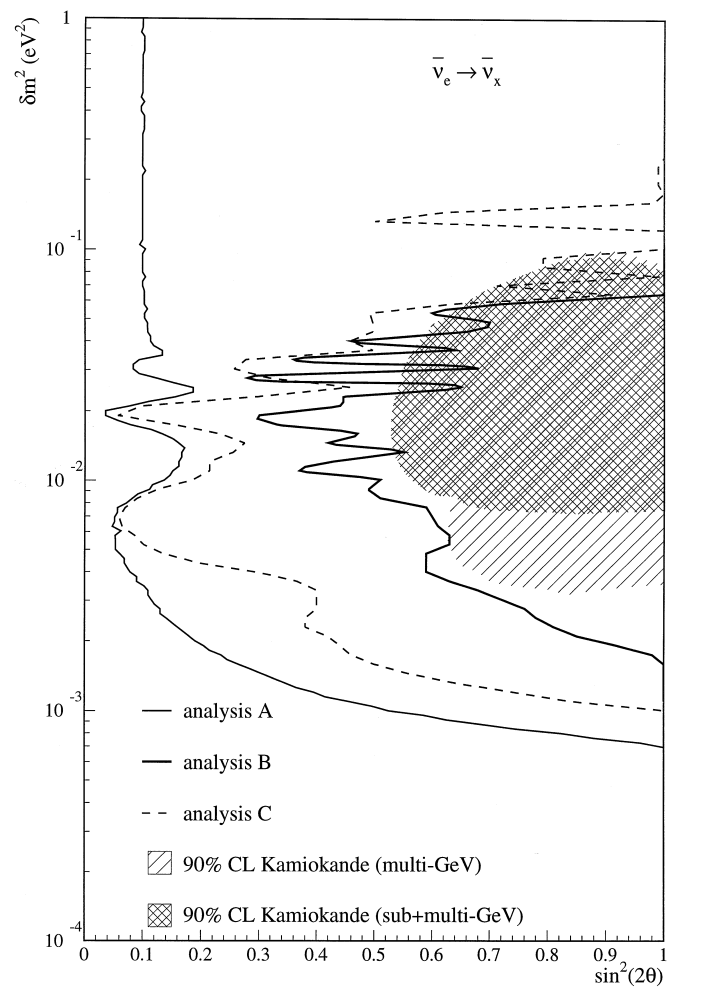
\includegraphics[height=0.5\textheight]{ch_introduction/chooz_exclusion}
    \caption{
        Exclusion contours for $\sin^22\thetaot$ and $\Delta m^2_{32}$
        at the end of the Chooz experiment \cite{chooz1999}.
        The hashed regions represent the exclusion contours
        based on Super-Kamiokande atmospheric measurements.
    }
    \label{fig:chooz_exclusion}
\end{figure}


There are numerous systematic uncertainties associated with the $\nu_\mu\to\nu_e$ appearance measurement
which have until the last decade or so been prohibitive.
For example, since the probability of $\nu_e$ appearance is so small,
just a few percent,
the proportion of the beam that is either $\nu_\mu$ or $\nu_\tau$ is large,
necessitating extremely accurate flavor identification of detected events.
A small false positive rate of mistaking $\nu_\mu$ events as $\nu_e$
would substantially bias the measurement.
Further, the composition of the neutrino beam must be known extremely well.
The standard method for neutrino beam production (\cref{subsec:nu_flavors})
also produces charged kaons, which decay to $e^\pm + (\nu_e/\nuebar)$
with a much larger branching ratio than the equivalent decay for pions.
Thus a measurement of $\nu_e$ appearance must be able to justify
that it is not simply observing $\nu_e$ that were produced directly
by the accelerator.

On the other hand, the disappearance measurement using reactor \nuebar{} is
free from many of the issues faced by the accelerator experiments.
With characteristic energies of \SIrange{1}{8}{\MeV},
any antineutrinos which oscillated into $\bar{\nu}_{\mu/\tau}$
would be below threshold for producing the associated charged lepton,
obviating the need for flavor identification.
Further, nuclear reactors produce neutrinos via $\beta^-$ decay,
thus producing only \nuebar{}.
The ideal interaction to observe these \nuebar{} events
is inverse beta decay (IBD),
which was used by Reines and Cowan in the first detection of (anti)neutrino events,
not coincidentally also from reactor \nuebar{} (\cref{subsec:discovery}).
As in the Reines and Cowan experiment,
modern reactor \nuebar{} experiments use liquid scintillator
as a detection medium.
Unlike in that earlier experiment, though,
modern experiments use liquid scintillator as the antineutrino target itself,
using organic scintillators with a large number of free protons
in the form of \isotope[1]{H}.
Systematic uncertainties arise in constraining the reactor \nuebar{} flux
and in accumulating sufficient statistics
so that any observed deficit of \nuebar{}
can be attributed to \thetaot{} rather than mis-modeling of the reactor
or a statistical fluctuation.

A new generation of reactor experiments
was designed to remedy the issue of reactor systematics
by constructing antineutrino detectors at both near and far sites
with respect to the reactor cores,
with the near detectors constraining the \nuebar{} flux prediction
and decreasing the systematic uncertainty.
The value of $\theta_{13}$ was first measured
with a significance of $\geq 5\sigma$
by the Daya Bay experiment in 2012 \cite{ngd2012},
followed closely by the RENO \cite{reno2012}
and Double Chooz \cite{doublechooz2012} experiments.
Accelerator experiments T2K and MINOS
searched for $\nu_\mu\to\nu_e$ (``$\nu_e$ appearance'')
and observed evidence for a nonzero \thetaot{}
as early as 2011 \cite{t2k2011,minos2011},
but only at a significance of $2\sigma$ to $3\sigma$.
Subsequent searches by accelerator experiments (e.g. \cite{t2k2018})
resulted in values of \thetaot{} which generally agree
with the reactor measurements.

Since the start of data taking on 24 December 2011,
the Daya Bay Reactor Neutrino Experiment has produced numerous measurements of
\thetaot{}, searches for sterile neutrinos \cite{dyb_sterile2020},
and the reactor \nuebar{} flux and spectrum \cite{dyb_spec_decomp2019},
and has also investigated
a variety of other physical phenomena (e.g. \cite{dyb_cpt2018}).
The Daya Bay measurement of \thetaot{} in April 2012
was the first nonzero measurement of that quantity
at a $5\sigma$ significance.
This measurement used 55 days of \nuebar{} data
and only six of the eight planned antineutrino detectors.
Since then, Daya Bay has published updated results using IBDs detected by
either neutron capture on gadolinium (nGd)
\cite{ngd2012,ngd2013,ngd2014,ngd2015,ngd2016,ngd2018}
or neutron capture on hydrogen (nH)
\cite{nh2014,nh2016}
as shown in \cref{fig:theta13_vs_t}.

\begin{figure}
    \centering
    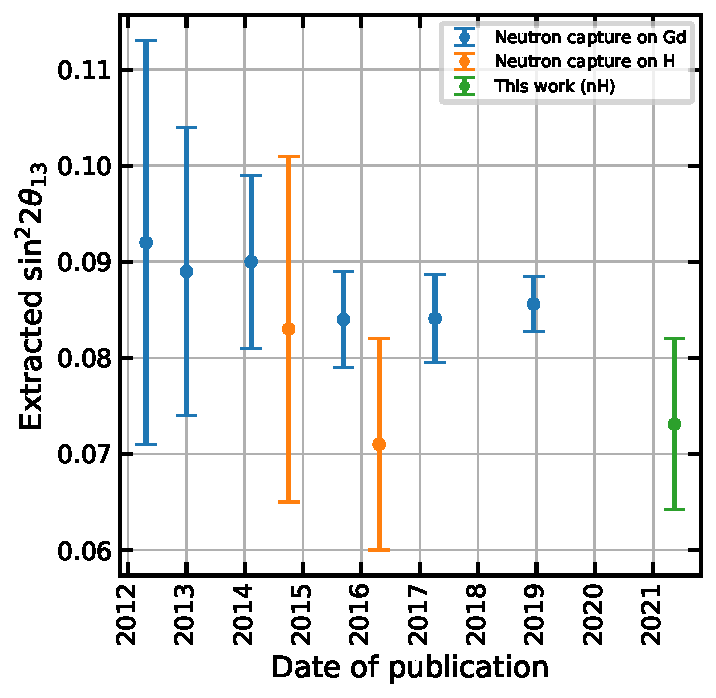
\includegraphics[height=0.4\textheight]{ch_detector/theta13_vs_time}
    \caption{
        Published values of $\sin^{2}2\thetaot$ over time
        for both nGd and nH analyses.
        Some nGd results were reported with separate statistical
        and systematic errors;
        those have been combined linearly for this plot.
        \todo[inline]{Include ``this work'' data point}
    }
    \label{fig:theta13_vs_t}
\end{figure}

This thesis will present a new measurement of \thetaot{}
based on observation of nH-IBD interactions
at the Daya Bay experiment,
with a focus on potential sources of the $\sim1\sigma$ discrepancy
between the nGd and nH extracted values for \thetaot{}.
The Daya Bay detector system is described in \cref{ch:detector}.
Calibration procedures and event reconstruction algorithms
are described in \cref{ch:calibration,ch:reconstruction}, respectively.
The procedure for selecting nH-IBD events and rejecting backgrounds
is described in \cref{ch:event_selection}.
In \cref{ch:simulation}, details of Monte Carlo simulation studies
will be presented.
\Cref{ch:analysis} will present the extraction of \thetaot{}
from the selected events.
